\newpage
\section{Wachstum und Zerfall}


\hfill \break
Algemeines:
$$f(x) = c*a^x$$
$$\textcolor{red}{N(t)} = \textcolor{blue}{N_0}*\textcolor{green}{a}^t$$

\begin{itemize}
    \item \textcolor{red}{$N(t)$}: Die Menge die zum Zeitpunkt t (noch) vorhanden ist.
    \item \textcolor{blue}{$N_0$}: Anfangsmenge oder Startwert.
    \item \textcolor{green}{$a$}: Wachstumes-Zerfallsfaktor.
    \item bei $a>1$ ist es ein Zuwachs
    \item bei $0<a<1$ ist es ein Verfall
\end{itemize}


\hfill \break
Umrechnung zwischen Funktionstypen:
$$N(t) = \textcolor{blue}{2}*\textcolor{red}{1.03}^t  \longrightarrow  N(t) = \textcolor{blue}{16}*\textcolor{red}{e^\lambda}^t$$

$$\fboxrule=0.8pt \fcolorbox{black}{lightgray}{%
        \begin{tabular}[t]{@{}l@{}}
            $1.03 = e^\lambda$ | /Ln      \\
            $Ln(1.03) = \lambda * L_e(e)$ \\
            $\lambda = 0.02855...$        \\
            $N(t) = 2*e^0.02855...$       \\
        \end{tabular}}$$


\hfill \break
Thermologie:
\begin{itemize}
    \item Halbwertszeit: Ist jene Zeit t, die vergehen muss bis nur noch die Hälfte des Anfangswetes vorhanden ist.
    \item Verdopplungszeit: Ist jene Zeit t, die vergehen muss bis das Doppelte des Anfangswetes vorhanden ist.
\end{itemize}

\break
\subsection{Modelle}

\hfill \break
Lineares Modell:\\
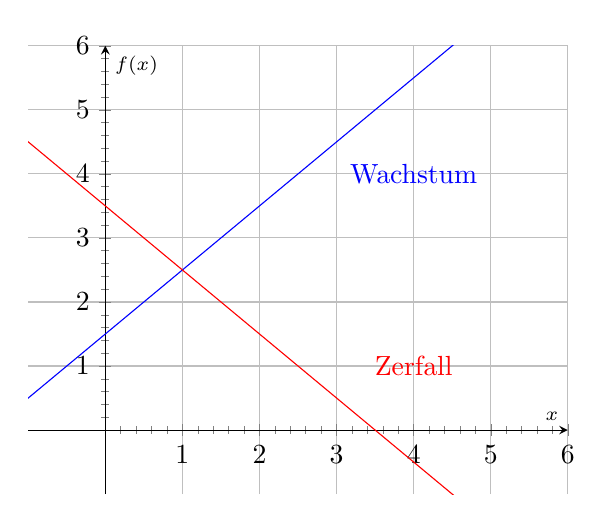
\begin{tikzpicture}[scale=1.0]
    \begin{axis}%
        [
            grid=major,
            xtick={0,1,...,7},
            minor x tick num=4, % 4 minor ticks => 5 subintervals
            xmin=-1,
            xmax=6,
            xlabel={\scriptsize $x$},
            axis x line=middle,
            ytick={0,1,...,7},
            minor y tick num=4,  % 4 minor ticks => 5 subintervals
            ymin=-1,
            ymax=6,
            ylabel={\scriptsize $f(x)$},
            axis y line=middle,
            no markers,
            samples=100,
            domain=-6:6,
        ]
        \addplot[blue] (x,{x+1.5});
        \addplot[red] (x,{-x+3.5});
        \node[color=blue] at (4,4) {Wachstum};
        \node[color=red] at (4,1) {Zerfall};
    \end{axis}
\end{tikzpicture}

\hfill \break
Exponentielles Modell:\\
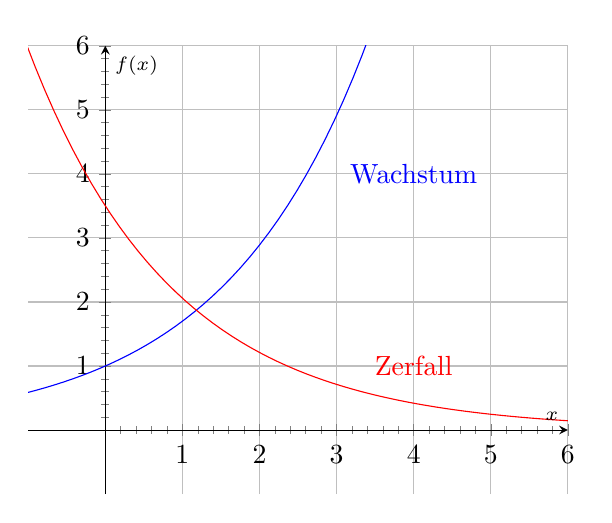
\begin{tikzpicture}[scale=1.0]
    \begin{axis}%
        [
            grid=major,
            xtick={0,1,...,7},
            minor x tick num=4, % 4 minor ticks => 5 subintervals
            xmin=-1,
            xmax=6,
            xlabel={\scriptsize $x$},
            axis x line=middle,
            ytick={0,1,...,7},
            minor y tick num=4,  % 4 minor ticks => 5 subintervals
            ymin=-1,
            ymax=6,
            ylabel={\scriptsize $f(x)$},
            axis y line=middle,
            no markers,
            samples=100,
            domain=-6:6,
        ]
        \addplot[blue] (x,{1.7^x});
        \addplot[red] (x,{3.5*(1.7^-x)});
        \node[color=blue] at (4,4) {Wachstum};
        \node[color=red] at (4,1) {Zerfall};
    \end{axis}
\end{tikzpicture}

\hfill \break
Beschränktes Wachstum:\\
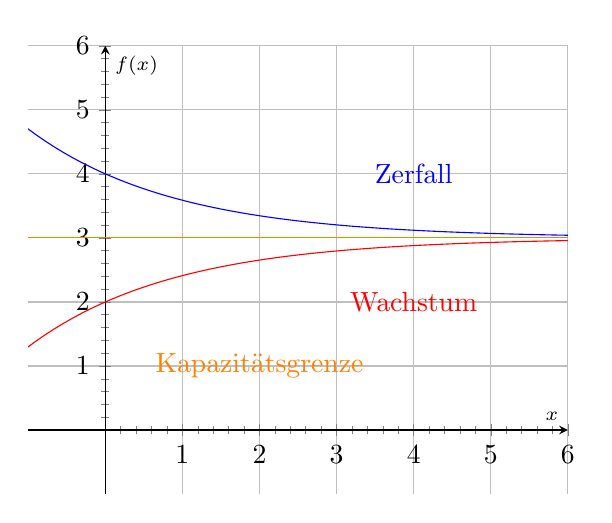
\begin{tikzpicture}[scale=1.0]
    \begin{axis}%
        [
            grid=major,
            xtick={0,1,...,7},
            minor x tick num=4, % 4 minor ticks => 5 subintervals
            xmin=-1,
            xmax=6,
            xlabel={\scriptsize $x$},
            axis x line=middle,
            ytick={0,1,...,7},
            minor y tick num=4,  % 4 minor ticks => 5 subintervals
            ymin=-1,
            ymax=6,
            ylabel={\scriptsize $f(x)$},
            axis y line=middle,
            no markers,
            samples=100,
            domain=-6:6,
        ]
        \addplot[blue] (x,{(1.7^-x)+3});
        \addplot[red] (x,{(-1.7^-x)+3});
        \node[color=blue] at (4,4) {Zerfall};
        \node[color=red] at (4,2) {Wachstum};
        \addplot[orange] (x,{3});
        \node[color=orange] at (2,1) {Kapazitätsgrenze};
    \end{axis}
\end{tikzpicture}

\hfill \break
Logisches Wachstum:\\
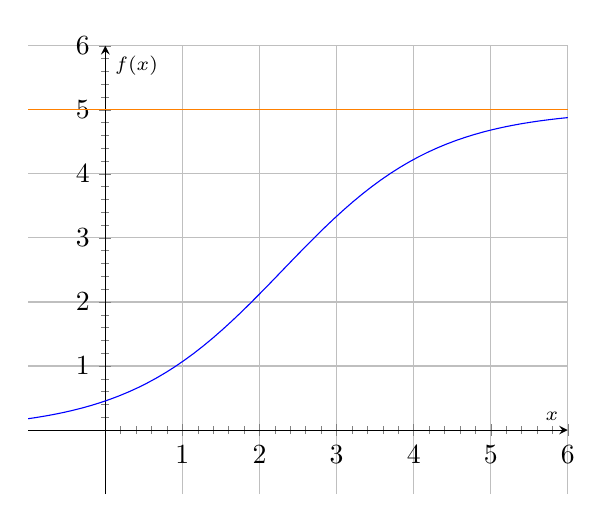
\begin{tikzpicture}[scale=1.0]
    \begin{axis}%
        [
            grid=major,
            xtick={0,1,...,7},
            minor x tick num=4, % 4 minor ticks => 5 subintervals
            xmin=-1,
            xmax=6,
            xlabel={\scriptsize $x$},
            axis x line=middle,
            ytick={0,1,...,7},
            minor y tick num=4,  % 4 minor ticks => 5 subintervals
            ymin=-1,
            ymax=6,
            ylabel={\scriptsize $f(x)$},
            axis y line=middle,
            no markers,
            samples=100,
            domain=-6:6,
        ]
        \addplot[orange] (x,{5});
        \addplot[blue] (x,{5/(1+10*e^-x)});
    \end{axis}
\end{tikzpicture}
\break
\newpage
\subsection{Lineares Modell}

\subsubsection{Wachstum}
\hfill \break
Es Ligen 25€ am Spaarbuch. Jede Woche werdern 5€ angespaart.
\hfill \break
$K(t)=\textcolor{red}{5}t+\textcolor{blue}{25}$

\begin{itemize}
    \item \textcolor{red}{5}: Zuanhme pro Woche (Konstant)
    \item \textcolor{blue}{25}: Startwert
\end{itemize}

\hfill \break
Darstellung:\\
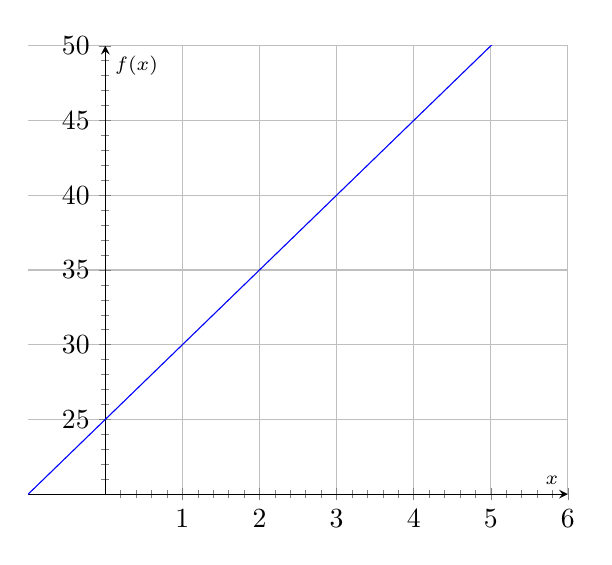
\begin{tikzpicture}[scale=1.0]
    \begin{axis}%
        [
            grid=major,
            xtick={0,1,...,7},
            minor x tick num=4, % 4 minor ticks => 5 subintervals
            xmin=-1,
            xmax=6,
            xlabel={\scriptsize $x$},
            axis x line=middle,
            ytick={20,25,...,50},
            minor y tick num=4,  % 4 minor ticks => 5 subintervals
            ymin=20,
            ymax=50,
            ylabel={\scriptsize $f(x)$},
            axis y line=middle,
            no markers,
            samples=100,
            domain=-6:6,
        ]
        \addplot[blue] (x,{5*x+25});
    \end{axis}
\end{tikzpicture}

\newpage
\subsubsection{Zerfall}

\hfill \break
Es Ligen 90€ auf einem Spaarbuch. Jede Woche werdern 5€ angehoben.
\hfill \break
$K(t)=\textcolor{red}{-5}t+\textcolor{blue}{90}$

\begin{itemize}
    \item \textcolor{red}{5}: Abnahme pro Woche (Konstant)
    \item \textcolor{blue}{25}: Startwert
\end{itemize}

\hfill \break
Darstellung:\\
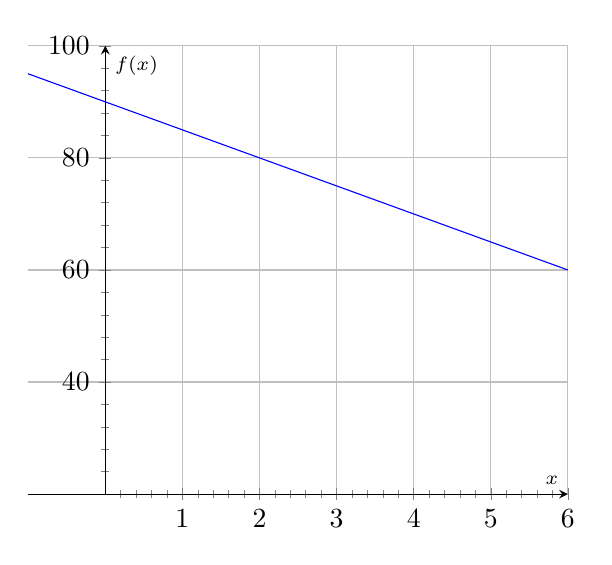
\begin{tikzpicture}[scale=1.0]
    \begin{axis}%
        [
            grid=major,
            xtick={0,1,...,7},
            minor x tick num=4, % 4 minor ticks => 5 subintervals
            xmin=-1,
            xmax=6,
            xlabel={\scriptsize $x$},
            axis x line=middle,
            ytick={20,40,...,100},
            minor y tick num=4,  % 4 minor ticks => 5 subintervals
            ymin=20,
            ymax=100,
            ylabel={\scriptsize $f(x)$},
            axis y line=middle,
            no markers,
            samples=100,
            domain=-6:6,
        ]
        \addplot[blue] (x,{-5*x+90});
    \end{axis}
\end{tikzpicture}
\break
\newpage
\subsection{Exponentielles Modell}

\subsubsection{Wachstum}
\hfill \break
Jemand hat 25€ am Spaarbuch und bekommt Wöchentich 3\% vom Ersparten dazu.
\hfill \break
$K(t)=\textcolor{red}{25}*\textcolor{blue}{1.03}^t$

\begin{itemize}
    \item \textcolor{red}{25}: Startwert
    \item \textcolor{blue}{1.05}: Wachstrumsfaktor
\end{itemize}

\hfill \break
Darstellung:\\
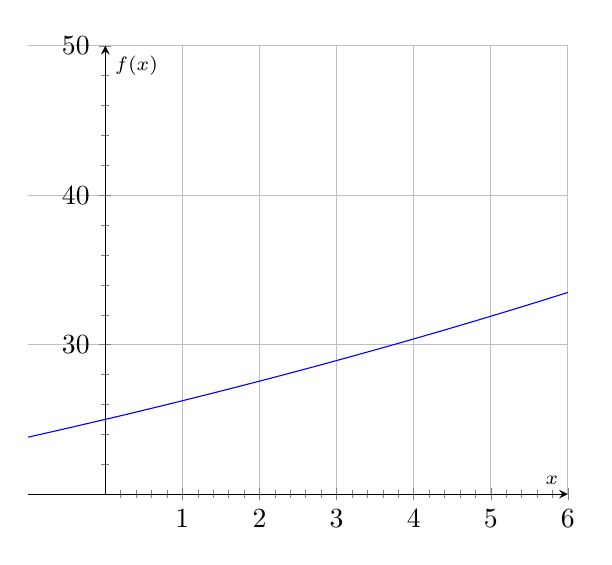
\begin{tikzpicture}[scale=1.0]
    \begin{axis}%
        [
            grid=major,
            xtick={0,1,...,7},
            minor x tick num=4, % 4 minor ticks => 5 subintervals
            xmin=-1,
            xmax=6,
            xlabel={\scriptsize $x$},
            axis x line=middle,
            ytick={10,20,...,50},
            minor y tick num=4,  % 4 minor ticks => 5 subintervals
            ymin=20,
            ymax=50,
            ylabel={\scriptsize $f(x)$},
            axis y line=middle,
            no markers,
            samples=100,
            domain=-6:6,
        ]
        \addplot[blue] (x,{25*1.05^x});
    \end{axis}
\end{tikzpicture}

\newpage
\subsubsection{Zerfall}

\hfill \break
Auf einem Konto Liegen 90€. Es werden monatlich 20\% abgehoben.
\hfill \break
$K(t)=\textcolor{red}{90}*\textcolor{blue}{0.80}^t$

\begin{itemize}
    \item \textcolor{red}{25}: Startwert
    \item \textcolor{blue}{0.80}: Zerfallsfaktor
\end{itemize}

\hfill \break
Darstellung:\\
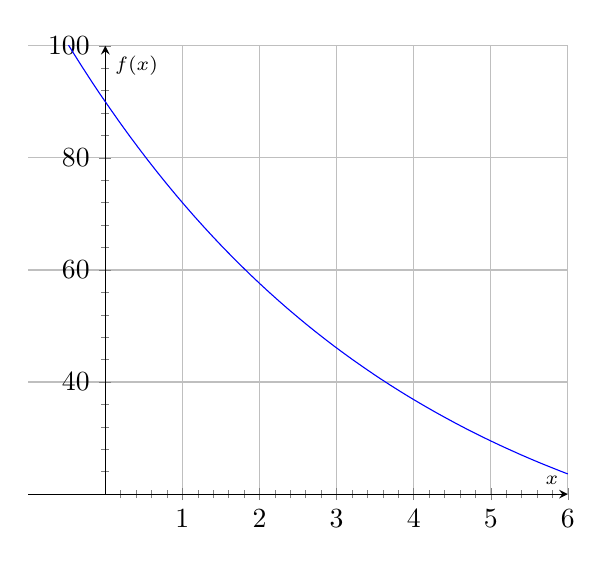
\begin{tikzpicture}[scale=1.0]
    \begin{axis}%
        [
            grid=major,
            xtick={0,1,...,7},
            minor x tick num=4, % 4 minor ticks => 5 subintervals
            xmin=-1,
            xmax=6,
            xlabel={\scriptsize $x$},
            axis x line=middle,
            ytick={20,40,...,100},
            minor y tick num=4,  % 4 minor ticks => 5 subintervals
            ymin=20,
            ymax=100,
            ylabel={\scriptsize $f(x)$},
            axis y line=middle,
            no markers,
            samples=100,
            domain=-6:6,
        ]
        \addplot[blue] (x,{90*0.80^x});
    \end{axis}
\end{tikzpicture}
